\documentclass[
	% -- opções da classe memoir --
	article,			% estilo de artigo
	12pt,				% tamanho da fonte
	openright,			% capítulos começam em pág ímpar (insere página vazia caso preciso)
	oneside,			% para impressão em verso e anverso. Oposto a twoside
	a4paper,			% tamanho do papel. 
	% -- opções da classe abntex2 --
	%chapter=TITLE,		% títulos de capítulos convertidos em letras maiúsculas
	%section=TITLE,		% títulos de seções convertidos em letras maiúsculas
	%subsection=TITLE,	% títulos de subseções convertidos em letras maiúsculas
	%subsubsection=TITLE,% títulos de subsubseções convertidos em letras maiúsculas
	% -- opções do pacote babel --
	english,			% idioma adicional para hifenização
	%french,				% idioma adicional para hifenização
	%spanish,			% idioma adicional para hifenização
	brazil				% o último idioma é o principal do 
	]{abntex2}

% ---
% PACOTES
% ---

% ---
% Pacotes fundamentais 
% ---
\usepackage{cmap}				% Mapear caracteres especiais no PDF
\usepackage{lmodern}			% Usa a fonte Latin Modern
\usepackage[T1]{fontenc}		% Selecao de codigos de fonte.
\usepackage[utf8]{inputenc}		% Codificacao do documento (conversão automática dos acentos)
\usepackage{indentfirst}		% Indenta o primeiro parágrafo de cada seção.
\usepackage{color}				% Controle das cores
\usepackage{graphicx}			% Inclusão de gráficos
\usepackage{multirow}			% Tabelas
\usepackage{nicefrac}			% Frações
% ---
\usepackage{enumerate}
\usepackage{array}
\usepackage{amsmath}
\usepackage{amsfonts}
\usepackage{amsthm}
\usepackage{scalefnt}
\usepackage{tabularx}
% ---
% Pacotes adicionais, usados apenas no âmbito do Modelo Canônico do abnteX2
% ---
\usepackage{lipsum}				% para geração de dummy text
%\usepackage[english,brazil]{babel}
% ---
\usepackage{makeidx}
\usepackage[margin=2.5cm]{geometry}
% ---
% Pacotes de citações
% ---
\usepackage[alf,bibjustif]{abntex2cite}	% Citações padrão ABNT (bibjustif) Forçar alinhamento à direita
% Page length commands go here in the preamble


\hypersetup{hidelinks}
\renewcommand{\baselinestretch}{1.0} % 1.5 denotes double spacing. Changing it will change the spacing



\date{}
\begin{document}
\title{Assimetria vertical de transmissão de preços no mercado de gasolina e o impacto da introdução da tecnologia \textit{flex-fuel}}
\author{Caio Matteucci de Andrade Lopes \thanks{caiolopes@ufpr.br} \\
  \text{UFPR}
  \and Lucas Lourenço Lopes \thanks{blablabla@ufpr.br} \\
   \text{UFPR}
  \and Marcos Minoru Hasegawa \thanks{blablabla@ufpr.br} \\
   \text{UFPR}}

\maketitle

\begin{abstract}
O objetivo deste trabalho é observar a existência de assimetria na transmissão de preços no mercado da gasolina, e analisar como se comportou esta transmissão com a introdução da tecnologia \textit{flex-fuel}. Para isso, se utilizou de um modelo autorregressivo com \textit{threshold} (TAR), que permite não-linearidades na análise da cointegração, capturando possíveis assimetrias de transmissão. Foram encontradas evidências de assimetria na transmissão dos preços no período pós introdução da nova tecnologia, mas não no período anterior, corroborando com a intuição de que houve mudança de estratégia no mercado de gasolina.    \\ \\
\textbf{Classificação JEL}: Q41, R15, C22 \\
\textbf {Palavras-chave}: Assimetria de transmissão, Ajustamento com \textit{threshold}, Processo autorregressivo com \textit{threshold}
\end{abstract}



%{ 
\selectlanguage{english}
\begin{abstract}

The objective of this work is to observe the existence of asymmetry in the transmission of prices in the gasoline market, and to analyze how this transmission behaved with the entry of the flex-fuel technology. In order to capture possible transmission asymmetries we used an autoregressive model with threshold (TAR), which allows nonlinearities in the cointegration analysis. Evidence of asymmetry in the transmission of prices in the post-introduction period of the new technology was found, but not in the previous period, corroborating with the intuition that there was a change of strategy in the gasoline market. \\ \\
\textbf{JEL classification}: Q41, R15, C22 \\
\textbf {Keywords}: Asymetric transmission, Threshold ajustment, Threshold autorefressive process

\end{abstract}
\selectlanguage{brazil}

\cleardoublepage
% ----------------------------------------------------------
% Introdução
% ----------------------------------------------------------
\section{Introdução}
\addcontentsline{toc}{chapter}{Introdução}

Estudos sobre a interação dos mercados e transmissão de preços são recorrentes na literatura econômica. Os primeiros estudos que se preocuparam com esse assunto analisaram apenas a correlação entre os preços, em cada mercado ou elo da cadeia produtiva, para explicar como se dava essa transmissão. O primeiro modelo que se preocupou com o caráter dinâmico dessas relações foi o proposto por \citeonline{Ravallion1986}, observando a diferença entre a relação de preços de curto prazo, da relação de equilíbrio de preços no longo prazo, como bem aponta \citeonline{Mattos2009}.

Conforme \citeonline{Garaffa2016}, modelos de forma reduzida (ou modelos financeiros) ganharam força ao longo dos anos 2000, devido ao processo de financeirização do mercado de commodities. Estes modelos diferem dos modelos estruturais ao focar na relação de interação entre os preços, não se preocupando com a estimação de parâmetros de oferta ou demanda. Desta forma, modelos na forma reduzida demandam apenas informações sobre as propriedades das séries históricas de preços, e se desenvolveram a partir dos modelos autorregressivos (AR), com posterior incorporação de dos modelos de correção de erro e análises de cointegração \apud{Huntington2013}{Garaffa2016}.

Neste trabalho será analisada a transmissão de preços da cadeia produtiva da Gasolina, nos níveis de distribuição e revenda, na cidade de Curitiba-PR, capital e maior cidade do estado. Para tal será utilizado método TVEC (\textit{Threshold Vector Errors Correction}), que é uma versão não linear do modelo de vetor de correção de erros (VEC), membro do grupo de modelos TAR, do inglês \textit{Threshold Autoregressive Models}.

Os modelos TAR apresentam um avanço em relação aos seus anteriores, lineares, no sentido de possibilitarem a incorporação da análise de assimetrias e custos de transação  ao arcabouço de estudo da integração de mercados. Estas imperfeições geram não-linearidades no movimento de ajuste de preços que não são captadas pelos modelos autorregressivos tradicionais. Vale apontar que esta classe de modelos, apesar de ser compatível com os conceitos de custos de transação e assimetrias, não é capaz de apontar a origem dos mesmos, apenas pode mensurar seus efeitos.

São exemplos de trabalhos que adotaram modelos com \textit{threshold} os trabalhos de \citeonline{Serra2006}, que tratam os custos de transação no mercado de porco europeu por meio do modelo TAR; \citeonline{Ben-Kaabia2007} que também por meio de um modelo TAR analisaram as assimetrias entre os preços ao produtor e varejista no mercado de carne de carneiro na Espanha; Nick e Threschler (2014), que observaram a aplicabilidade da lei do preço único no mercado de gás natural europeu por meio de um modelo TVEC; \citeonline{Mattos2009}, que por meio de um modelo TVEC analisou os custos de transação no mercado do boi gordo brasileiro e, no mesmo ano, com uso de um modelo TAR, analisou os custos de transação no mercado de frango do Brasil; Garaffa (2016), em consonância com o trabalho de Nick e Theschler (2014) avalia o mercado de gás europeu por meio de modelos TVEC e TVAR e; \citeonline{Abdulai2002} por meio de um modelo TAR observa a transmissão de preços ao longo da cadeia do mercado de carne suína suíço, ou seja, analisa também a transmissão vertical de preços.

Em linha mais semelhante ao objetivo deste trabalho, temos o estudo de \citeonline{Chen2005} que, com uso de um modelo TAR com especificação alternativa, buscou identificar a assimetria de transmissão de preços na cadeia produtiva da gasolina, considerando os mercados \textit{spot} e futuro, dividindo a cadeia em duas partes, uma do petróleo até a refinaria, e outra da refinaria até a venda final da gasolina. Suas principais conclusões apontam para a presença de assimetria em ambos os mercados, \textit{spot} e futuro, mas com  assimetria significativa apenas na segunda parte da cadeia.

O objeto deste trabalho será o mercado de combustíveis de Curitiba-PR. Podemos dizer que tal escolha se justifica pela importância da questão energética, tanto em âmbito nacional como internacional, e no fato de que Curitiba, como capital  maior cidade do Estado do Paraná, poder apresentar bons indícios de como este mercado se comporta em nível metropolitano ou mesmo estadual.  Além disso, o assunto se torna relevante pela introdução da tecnologia \textit{flexfuel} no mercado automobilístico nacional em meádos dos anos 2000, incluídos no período de análise. Este acontecimento pode ter influenciado a forma como os preços de combustível interagem tanto ao longo da cadeia, verticalmente, como entre mercados, horizontalmente.

O texto está organizado em 6 seções, além desta primeira, introdutória. A segunda seção traz os objetivos desta pesquisa, bem como sua relevância. A terceira, consiste na análise descritiva dos dados. Na seção 4, é desenvolvida a metodologia do trabalho. Na quinta seção, são apresentados os resultados e interpretação da estimação do modelo. Por fim, a última seção apresenta as conclusões encontradas neste trabalho.

% ----------------------------------------------------------
% Capitulo de textual  
% ----------------------------------------------------------
\section{Objetivos}

O objetivo principal deste trabalho é analisar a relação de transmissão de preços entre distribuidores e revendedores de combustíveis - especificamente gasolina tipo C, no município de Curitiba. Para tal, empregou-se a metodologia de Cointegração com \textit{threshold} e testou-se a presença de assimetria na transmissão de preços. Nesse contexto uma pergunta interessante surge: como a entrada de veículos com a tecnologia \textit{flexfuel} pode ter alterado (ou não) a transmissão vertical de preços do mercado analisado? 

% ----------------------------------------------------------
% Capitulo de textual  
% ----------------------------------------------------------
\section{Dados}

Estes dados foram disponibilizados pela Superintendência de Planejamento e Pesquisa no sítio da ANP e refletem o preço de venda médio (por litro) de gasolina tipo C realizadas pelas distribuidoras e revendedoras dos derivados combustíveis de petróleo no município de Curitiba. O período de análise é de janeiro de 2003 à dezembro de 2012, entretanto, a fim de melhorar a precisão da análise e facilitar a comparação dos resultados, este período é dividido em dois subperíodos, em função da influência sofrida pela entrada da tecnologia flex fuel no mercado.

Os valores mensais correntes foram deflacionados utilizando a série histórica do Índice Nacional de Preços ao Consumidor (IPCN), disponibilizada no sitio do Instituto Brasileiro de Geografia e Estatística, IBGE. Foi utilizado o mês de fevereiro de 2016 como referência para os cálculos.

\begin{figure}
    \caption{Gráfico dos Preços de Revenda e Distribuição \label {ker}}
    \centerline{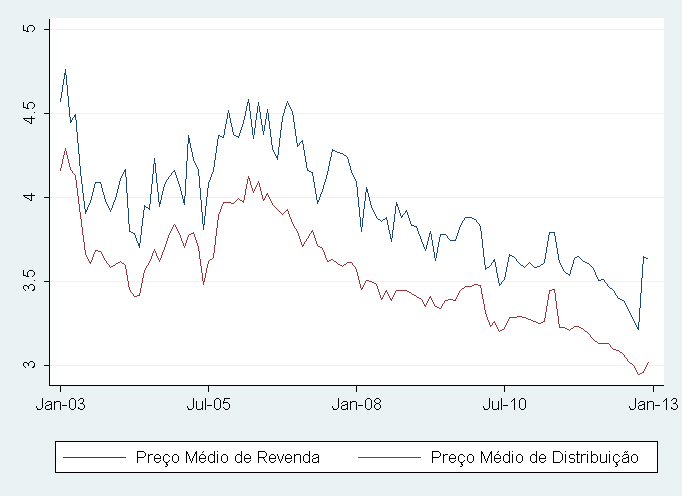
\includegraphics[width=18cm, height=10cm]{precos.png}}
\end{figure}



% ----------------------------------------------------------
% Capitulo de textual  
% ----------------------------------------------------------
\section{Metodologia}


Modelos que examinam a natureza da transmissão vertical de preços foram analisados em diferentes mercados, mas principalmente no setor alimentício. Esta relação começou a ser estudada pelo modelo de \citeonline{Houck1977} passou por diversas modificações com o passar do tempo. Seja o modelo estático na forma reduzida dado por:

\begin{equation} \label{rer}
\sum_{\tau=1}^{t} \Delta PR_{\tau}=\alpha_{0} + \alpha_{1}\sum_{\tau=1}^{t}\Delta PPI_{\tau} + \alpha_{2}\sum_{\tau=1}^{t}\Delta PPF_{\tau} + \varepsilon_{t}
\end{equation}


Em que $PR_{\tau}$ representa variações nos preços do revendedor, $PPI_{\tau}$ e $PPF_{\tau}$ são as variações positivas e negativas nos preços de distribuição/produção, respectivamente, $\alpha_{0}$, $\alpha_{1}$ e $\alpha_{2}$ são coeficientes a serem estimados, $t$ é o tempo corrente e $\varepsilon_{t}$ é o termo de erro aleatório. A hipótese nula de ajuste simétrico de preços é testada por meio das estimativas de $\alpha_{1}$ e $\alpha_{2}$. É comum o uso de técnicas de cointegração para estimar estes parâmetros, entretanto, \citeonline{Cramon-Taubadel1996} demonstraram que a especificação na equação \ref{rer} é inconsistente com o conceito de cointegração. Em seguida, \citeonline{Azzam1999}, em um  trabalho seminal, mostrou que, na presença de rigidez de preço, com uso de funções não reversíveis, como é o caso da equação \ref{rer}, o teste de assimetria não é apropriado.

Nesse sentido, este trabalho emprega um modelo de cointegração que reconhece o fato de que um choque pode ter que atingir um nível crítico antes que uma resposta significativa seja provocada. Considere a relação simples que é usada como base para várias análises de cointegração:

\begin{equation}
\Delta x_{t}=\pi x_{t-1} + \vartheta_{t}
\end{equation}

Em que $x_{t}$ é um vetor de variáveis estacionárias não aleatórias, $\pi$ é uma matriz $n x n$, e $\vartheta_{t}$ é um componente de erro normalmente distribuído. O procedimento de cointegração de Johansen consiste em estimar $\pi$ e determinar seu rank. A idéia dessa abordagem é testar se o rank de $\pi$ é ou não igual a zero. Em caso negativo, o sistema exibe ajustamento simétrico em torno de $x_{t}=0$, ou seja, para qualquer $x_{t}\neq 0$, $\Delta x_{t+1}$ será igual à $\pi x_{t}$.


A abordagem de dois passos de \citeonline{Engle1987} também testa o ajuste simétrico. Para isso, utiliza o método OLS para estimar a relação de equilíbrio de longo prazo, como:

\begin{equation} \label{wfw}
x_{1t}=\beta_{0}+\beta_{2}x_{2t}+...+\beta_{n}x_{nt}+\mu_{t}
\end{equation}

Em que $x_{it}$ são variáveis não estacionárias, $\beta_{i}$ são parâmetros a ser estimados e $\mu_{t}$ é um termo de erro que pode apresentar correlação serial. Os resíduos são utilizados para estimar a seguinte relação:

\begin{equation} \label{acf}
\Delta \mu_{t}=\rho \mu_{t-1}+\varepsilon_{t}
\end{equation}

Em que $\varepsilon_{t}$ é um ruído branco. A rejeição da hipótese nula de não cointegração (isto é, aceitando a hipótese alternativa de $2<\rho <0$) implica que os resíduos na Equação 3 são estacionários com média zero. De acordo com o teorema de \citeonline{Engle1987}, se $\rho \neq 0$, \ref{wfw} e \ref{acf} implica na existência de um modelo de correção de erros que pode ser representado por:

\begin{equation} \label{deo}
\Delta x_{1t}=\delta_{j}\left ( x_{1t-1}-\beta_{0}-\beta_{2t-1}-...-\beta_{n}x_{nt-1} \right ) + \sum_{j=1}^{k}\beta_{2j}\Delta x_{2,t-j}+...+\sum_{j=1}^{k}\beta_{nj}\Delta x_{n,t-j}+\upsilon_{1t}
\end{equation}

Em que $k$ determina a defasagem e $\upsilon_{1t}$ é um ruído branco. O termo dentro entre parênteses fornece o mecanismo de correção de erro. \citeonline{Enders1998} argumentam que os testes de cointegração de Engle-Granger e Johansen são mal especificados se o ajuste é assimétrico. Quando esses testes são empregados para analisar a transmissão de preço de uma relação vertical de um mercado, a hipótese implicita é que as respostas as variações de preços são simétricas: choques no preço de produção/distribuição geram variações da mesma magnitude no preço dos revendedores, independente do choque ser positivo ou negativo.

\citeonline{Enders1998} consideram um modelo alternativo de correção de erro denominado modelo autorregressivo com \textit{threshold} (TAR), no qual a Equação \ref{acf} é representada como:

\begin{equation} \label{dess}
\Delta \mu_{t}=\left\{\begin{matrix}
\rho_{1}\mu_{t-1}+\varepsilon_{t} \ \ \ \text{if} \ \ \ \mu_{t-1}\geq 0 \\ 
\rho_{2}\mu_{t-1}+\varepsilon_{t} \ \ \ \text{if} \ \ \ \mu_{t-1}<  0
\end{matrix}\right.
\end{equation}

A condição necessária para $\left \{ \mu_{t} \right \}$ ser estacionária é $-2<(\rho_{1},\rho_{2})<0$. \citeonline{Enders1998} mostram que se a seqüência é estacionária, as estimativas por OLS de $\rho_ {1}$ e $\rho_ {2}$ têm uma distribuição normal assintótica multivariada. O processo de ajuste é então formalmente quantificado como por meio da função indicadora:

\begin{equation} \label{des}
\Delta \mu_{t}=I_{t}\rho_{1}\mu_{t-1} +\left ( 1-I_{t} \right )\rho_{2}\mu_{t-1}+\varepsilon_{t}
\end{equation}

Tal que:
\begin{equation} \label{fei}
I_{t}=\left\{\begin{matrix}
1 \ \ \ \text{if} \ \ \ \mu_{t-1}\geq 0 \\ 
0 \ \ \ \text{if} \ \ \ \mu_{t-1}<  0
\end{matrix}\right.
\end{equation}


Nesse caso, zero representa o valor do \textit{threshlod}. Modelos que utilizam as equações \ref{des} e \ref{fei} são referidos como modelos de auto-regressão com \textit{threshold} (TAR), enquanto o teste para comportamento de equilibrio de longo prazo com \textit{threshold} é denominado teste de cointegração com \textit{threshold}. Assumindo que o sistema é convergente, $\mu_{t}=0$ é considerado o valor de equilibrio de longo prazo da série. Se $\mu_{t}$ está abaixo do valor de equilibrio, o ajustamento é de $\rho_{1}\mu_{t}$, por outro lado, Se $\mu_{t}$ está acima do valor de equilibrio, o ajustamento é de $\rho_{2}\mu_{t}$ 

Desta forma, se o ajuste é simétrico temos que $\rho_{1}=\rho_{2}$, ou seja,  a abordagem de Engle-Granger é um caso especial das Equações \ref{des} e \ref{fei}. Dada a existência de um vetor de cointegração, a representação do modelo de correção de erro apresentada em \ref{deo} pode ser escrita como:

\begin{equation} 
\Delta x_{1t}=\rho_{1.1}I_{t}\mu_{t-1}+\rho_{2.1}(1-I_{t})\mu_{t-1}+\sum_{j=1}^{k}\beta_{2j}\Delta x_{2,t-j}+...+\sum_{j=1}^{k}\beta_{nj}\Delta x_{n,t-j}+\upsilon_{1t}
\end{equation}

Em que $\rho_{1.1}$ e $\rho_{2.1}$ são os coeficientes de ajustamento para diferenças positivas e negativas, respectivamente. \citeonline{Enders1998} mostraram que a equação \ref{des} pode ser extendido para um modelo de defasagens em diferenças, como:

\begin{equation} \label{fea}
\Delta \mu_{t}=I_{t}\rho_{1}\mu_{t-1} +\left ( 1-I_{t} \right )\rho_{2}\mu_{t-1}+\sum_{i=1}^{\rho-1}\gamma_{i}\delta \mu_{t-i} +\varepsilon_{t}
\end{equation}

Em vez de estimar a equação \ref{des} por meio da função indicadora \ref{fei}, o \textit{threshold} pode ser determinado pela variação de $\mu_{t}$. Nesse caso, a função indicador fica:

\begin{equation} \label{odi}
I_{t}=\left\{\begin{matrix}
1 \ \ \ \text{if} \ \ \ \Delta\mu_{t-1}\geq 0 \\ 
0 \ \ \ \text{if} \ \ \ \Delta\mu_{t-1}<  0
\end{matrix}\right.
\end{equation}


De acordo com \citeonline{Enders1998}, a substituição de \ref{fei} por \ref{odi} é especialmente valiosa quando o ajuste é assimétrico, de modo que a série exibe mais "momentos" em uma direção do que em outras. Modelos estimados usando as Equações 3, \ref{res} e \ref{odi} são denominados modelos autorregressivos \textit{momentum-threshold} (M-TAR).

No modelo TAR, se, por exemplo, $-2<\rho_{1}<\rho_{2}<0$ a fase negativa da sequênica $\{\mu_{t} \}$ deverá ser mais persistente que a fase positiva. Enquanto no modelo M-TAR, se, por exemplo $|\rho_{1}|<|\rho_{2}|$, então o modelo apresenta menos variações positivas que negativas para $\Delta \mu_{t-1}$.

As estatísticas de teste para a hipótese nula $(\rho_{1}=\rho_{2}=0)$ usando a especificação TAR e M-TAR  são chamadas $\Phi_{\mu}$ e $\Phi_{\mu}^{*}$, respectivamente. Três fatores principais determinam as distribuições de $\Phi_{\mu}$ e $\Phi_{\mu}^{*}$. Estes incluem o número de defasagens de $\mu_{t}$ na Equação \ref{fea}, o número de variáveis e o tipo de elementos determinísticos incluídos na relação de cointegração. Os valores críticos apropriados para $\Phi_{\mu}$ e $\Phi_{\mu}^{*}$ são apresentados em \citeonline{Enders1998}.

% ----------------------------------------------------------
% Capitulo de textual  
% ----------------------------------------------------------
\section{Resultados}

A hipótese de que as séries de preços analisadas possuem raiz-unitária, é testada pelo método Dickey-Fuller aumentado (ADF). O teste de critério de informação AIC foi utilizado para determinar a defasagem apropriada das séries. Encontrou-se que uma defasagem é a mais apropriada para ambas as variáveis em análise. Para o período completo, ou seja, de janeiro de 2003 à dezembro de 2012, o valores da estatística do teste para os preços de revenda são $-3,142$ e $-8,070$ para e série em nível e em primeira diferença, respectivamente, enquanto a estatística do teste para os preços de distribuição são $-3,004$ e $-7,040$ para e série em nível e em primeira diferença, respectivamente, sendo que o valor crítico de $-3,99$ a 1\% de significância sugere que as duas séries tornam-se estacionárias após a primeira diferença.

Para assegurar que a série em primeira diferença é estacionária foi realizado, também, o teste DF-GLS.
O teste DF-GLS, apresentado por \citeonline{Elliott1996}, é uma versão atualizada do teste ADF padrão, proposto por \citeonline{Dickey1979}, para quando os dados apresentam média desconhecida e tendência.\footnote{Os autores mostraram, por meio de um \textit{Monte Carlo}, que o DF-GLS tem maior poder e performance em pequenas amostras.} Os resultados foram ao encontro do teste ADF indicando que todas as séries são integradas de primeira ordem.  O teste DG-GLS, por ter mais poder que o teste ADF, fornece um argumento mais forte para a estacionaridade da primeira diferença. O resultado completo dos testes porde ser observado na tabela \ref{raizunitaria}:


 \begin{table}[htbp]
   \centering
  \caption{Testes de Raiz Unitária}
    \begin{tabular}{c|l|c|c}
 \toprule
                   &       &  \multicolumn{1}{c}{ADF} & \multicolumn{1}{c}{DF-GLS}   \\ \hline \hline
   		Jan 2003	& $PR_{t}$				&  -3,142 (-3.99)	& -2,830 (-3,46)   		\\
         	à			& $PD_{t}$ 			&  -3,004 (-3.99) 	& -2,483 (-3,46)  		\\
         	Dez 2012	& $\Delta PR_{t}$		&  -8,070 (-3.99)  	& -5,720 (-3,46) 	   	\\
  					& $\Delta PD_{t}$		&  -7,040 (-3.99) 	& -4,941 (-3,46)              	\\  \hline
   	  	Jan 2003	& $PR_{t}$				& -3,722 (-4.04)	& -2,458 (-3,58)	   		\\
  		à			& $PD_{t}$ 			& -3,109 (-4.04) 	& -2,082 (-3,58)     	   	\\
  		Dez 2007	& $\Delta PR_{t}$		& -5,413 (-4.04)	& -4,725 (-3,58)    	   	\\
  					& $\Delta PD_{t}$		& -4,303 (-4.04)	& -3,738 (-3,58)  	        \\  \hline       	
		Jan 2008	& $PR_{t}$				& -3,527 (-4.04)	& -3,320 (-3,58)	   	        \\  		
  		à			& $PD_{t}$ 			& -3,281 (-4.04)   	& -3,376 (-3,58)	  	 	\\
		Dez 2012	& $\Delta PR_{t}$		& -6,046 (-4.04)	& -3,908 (-3,58)  	   	\\
					& $\Delta PD_{t}$		& -6,460 (-4.04)   	& -4,687 (-3,58)   	   	\\  \hline          \bottomrule
    \end{tabular}
  \label{raizunitaria}
\end{table}

   
  
Verificado que as séries são integradas de mesma ordem, passou-se para a análise de cointegração. Temos que a regressão de cointegração é especificada como:

\begin{equation} \label{rre}
PR_{t}=\beta_{0}+\beta_{1}PD_{t}+\mu_{t} 
\end{equation}


Em que $PR_{t}$ é o preço de revenda, $PD_{t}$ representa o preço de distribuição e $\mu_{t}$ são os resíduos que, caso sejam estacionários, garantem a relação de longo prazo entre os preços. Para a análise de cointegração \textit{à la} Engle-Granger, a equação \ref{rre} foi estimada por OLS. A estimativa da relação de equilibrio de longo prazo (com as estatísticas do teste t em parênteses) é dada por:


\begin{equation} \label{rrt}
PR_{t} = \underset{0.474}{0.106} + \underset{15.878 }{1.083}PD_{t} + \widehat{\mu}_{t}
\end{equation}



Seguindo o procedimento de Engle Granger, os resíduos da Equação \ref{rrt} são usados para estimar:

\begin{equation} \label{res}
\Delta\widehat{\mu}_{t}=\rho_{1}\widehat{\mu}_{t-1}+\gamma_{1}\Delta\widehat{\mu}_{t-1}+ \varepsilon_{t} 
\end{equation}

O valor estimado de $\rho_{1}$ é de $ -0,468$ e a estatística t para a hipótese nula, $\rho_{1}$=0, é de $-4,604$ os valores críticos para o procedimento de Engle-Granger são  $-1,62$, $-1,95$,  $-2,58$ para 10\%, 5\% e 1\%, respectivamente. Portanto, procedimento de Engle-Granger sugere que as duas séries de preços são cointegradas.  

Tanto o modelo TAR quanto o M-TAR podem ser formulados para diferentes especificações de defasagem. A escolha de nenhuma defasagem em ambos os casos foi feita pelo critério de informação AIC e BIC, já que o resultado não foi diferente. O modelo de cointegração com \textit{threshold} proporcinou uma estatística $\Phi_\mu$ de $22,298$ e $20,294$  no modelo TAR e M-TAR, respectivamente. Portanto, a hipótese nula de $\rho_{1}=\rho_{2}=0$ pode ser rejeitada à um nível de significância de 1\%, o que indica que as séries são cointegradas.

Sendo assim, a hipótese nula de ajustamento assimétrico de preços $(\rho_{1}=\rho_{2})$ pode ser testado por meio de um teste F padrão. A estatística F de $4,074$ no modelo TAR e de $1,465$ no modelo M-TAR indicam que não se pode rejeitar a hipótese nula de ajustameto simétrico dos preços no modelo M-TAR, mas é possível rejeitar a hipótese nula à 5\% no modelo TAR. 

\citeonline{Enders1998} mostram que em um modelo TAR, como das equações \ref{dess} e \ref{des}, se $-2< (\rho_{1}, \rho_{2})<0$, o valor do \textit{threshold} pode ser tal que o equilibrio de longo-prazo ocorra em $\mu_{t-1}=\lambda$. Sendo esse o resultado obtido tanto no modelo TAR quanto no M-TAR, o método de Chan (1993) foi, portanto, empregado para determinar uma estimativa consistente do \textit{threshold}. O valor de $-0,088$ foi obtido no modelo TAR e $0,007$ modelo no modelo M-TAR. O modelo TAR consistente, C.TAR, sugere que é possível rejeitar a hipótese nula de ajustamento simétrico de preços à $5\%$ de significância. Vale ressaltar que, pelos critério de informação AIC e BIC, o C.TAR apresentou o melhor ajustamento aos dados. Os resultados dos quatro modelos - TAR, \textit{momentum-threshold} (M-TAR), TAR consistente (C.TAR) e \textit{momentum-threshold} consistente (C.MTAR) -  podem sem observados pela tabela \ref{coint}.

\begin{table}[htbp]
   \centering
  \caption{Estimativas Modelo TAR por período}
    \begin{tabularx}{\textwidth}{X||l|c|c|c|c}
 \toprule
                   &       &  \multicolumn{1}{c}{TAR} & \multicolumn{1}{c}{MTAR} & \multicolumn{1}{c}{C.TAR}  & \multicolumn{1}{c}{C.MTAR} \\ \hline \hline
   					& $\rho_{1}$			&  -0,395 (-3,797) & -0,438(-4,016) &	-0,401 (-4,224) & -0,409 (-3,550) \\
         				& $\rho_{2}$ 			&  -0,739 (-5,493) & -0,644 (-4,945) & -0,868(-5,459) & -0,647 (-5,359) \\
         	Jan 2003	& $\rho_{1}=\rho_{2}$	&  4,074 (0,045)   & 	1,465 (0,228)  & 	6,356 (0,013) &  2,015 (0,158)    \\
  		à			& AIC 					&	-208,666 	  &  -204,278         & 	-211,4		& -204,774           \\
    		Dez 2012	& BIC 					&	-200,648 	  &  -196,259         & 	-203,382	& -196,755           \\
    					& \textit{THR} 			&	0		 	  &  0		         & 	-0,088		& 0,007           \\
    					& $\Phi_{\mu}$ 			&     	 22,298	  &      20,294 	   &	23,82		& 20,66		 \\   \hline
   		        		& $\rho_{1}$			&  -0,426 (-2,78)  & -0,422 (-2,677)  & -0,376 (-2,78) & -0,407(-2,651) \\
         				& $\rho_{2}$ 			&  -0,658 (-3,668) & -0,648 (-3,689) & -0,875 (-4,191) & -0,692 (-3,784) \\
         	Jan 2003	& $\rho_{1}=\rho_{2}$	&  0,972 (0,328)		 & 0,918 (0,342)	  & 4,021 (0,049) & 1,345 (0,251) \\
  		à			& 	AIC 				&  -70,202 		  & -69,603    	 & -74,449 		& -70,288 \\
  		Dez 2007	& 	BIC 					&  -64,651    	 & -64,053    	 & -68,899		& -64,737 \\
  					& \textit{THR}			&  0   			 &  0  	 		  & -0,106		& -0,02     \\		
    					& $\Phi_{\mu}$ 			&  10,593    			& 10,387		  & 12,649		& 10,676   \\    \hline       	
          				& $\rho_{1}$	   	&  -0,493 (-3,026) & -0,422 (-2,677)  & -0,438 (-2,895) & -0,395 (-2,332) 		\\
         				& $\rho_{2}$ 		& -0,897(-4,057)	 & -0,648 (-3,689)   & -1,111 (-4,720)	 &  -0,911 (-4,322) 		\\
		Jan 2008	& $\rho_{1}=\rho_{2}$	&   2,162 (0,146)	 & 0,056 (0,812)	&  5,779 (0,019)      & 3,647 (0,061)         \\  		
  		à			& 	AIC 				&   -110.783   		 & -108,033		    & -115,995		 & -70,288     \\
		Dez 2012		& 	BIC 					&  -105.233			 &  -102,482  		   &	-110,445 	 & -64,737	 \\
					& \textit{THR}			&  0   				 & 0    			    & -0,044  			 & -0,02         \\  	
    					& $\Phi_{\mu}$ 			&  12,806			 &  9,647 		    & 15,331		       & 12,059               \\    \hline         
 \bottomrule
    \end{tabularx}
  \label{coint}
\end{table}


A possibilidade de um ajuste assimétrico de preços encontrado pelo modelo C.TAR implica que é incorreto examinar a dinâmica de curto prazo com um modelo simétrico de correção de erros. Um modelo simétrico de correção de erros não revelaria ajustes diferenciais das mudanças positivas e negativas (Enders e Granger, 1998). Assim, o modelo de correção de erro assimétrico (modelo C.TAR) é empregado na análise. Ele pode ser representado como:

\begin{equation}
\Delta PR_{t}=\sum_{s=1}^{k}\alpha_{s}\Delta PR_{t-s}+\sum_{s=0}^{k}\beta_{s}\Delta  PD_{t-s}+\gamma_{1}Z_{t-1}^{pos}+\gamma_{2}Z_{t-1}^{neg}
\end{equation}

Em que $k$ é a defasagem, $Z_{t-1}^{pos}$ e $Z_{t-1}^{neg}$ São os termos de correção de erro das regressões da cointegração com \textit{threshold}, representando ajustes de choques positivos e negativos às variações na margem de comercialização. Estes termos podem ser representados da seguinte forma:

\begin{align*}
Z_{t-1}^{pos}&=I_{t}\left (PR_{t-1}+0.164-1.216PD_{t-1} \right )\nonumber \\
Z_{t-1}^{neg}&=\left (1-I_{t}\right )\left (PR_{t-1}+0.164-1.216PD_{t-1} \right ) \nonumber
\end{align*}

Em que $I$ é uma função indicadora. A tabela \ref{ecm} apresenta os resultados do modelo de correção de erros. As estimativas do modelo simétrico e assimétrico foram apresentadas para a comparação. Vale ressaltar que as estatísticas t para $Z_{t-1}^{pos}$ e $Z_{t-1}^{neg}$ sugerem que o preço de revenda não responde a choques positivos na margem de comercialização, mas responde a choques negativos a $5\%$ de significância.

Para avaliar o efeito da entrada dos carros \textit{flexfuel} no contexto da transmissão de preços de gasolina entre revendedora e distribuidora vamos repetir as duas análises - cointegração com \textit{threshold} e modelo de correção de erro assimétrico (e simétrico) - em dois períodos distintos: de janeiro de 2003 à dezembro de 2007 e de janeiro de 2008 à dezembro de 2012.

Em ambos os períodos, os resultados sugerem que o modelo C.TAR é a especificação que melhor se ajusta aos dados. É possível rejeitar a hipótese nula de não cointegração $(\rho_{1}=\rho_{2}=0)$ à $1\%$ em todas especificações e para todos os períodos. A hipótese nula de ajustamento assimétrico de preços $(\rho_{1}=\rho_{2})$ também foi testada. Analisando o modelo C.TAR, no período em que haviam menos veículos \textit{flexfuel} no mercado, de 2003 a 2007, a estatística F encontrada foi de $4,021$ e o p-valor de $0,049$. No periódo seguinte, a estatística F calculada subiu para $5,779$ e o p-valor foi de $0,019$. Ou seja, pode-se rejeitar a hipótese nula de ajustamento simétrico de preços à $5\%$ de significância, em ambos os casos. 

Entretanto, vale ressaltar a redução de $3$ pontos percentuais no p-valor de um período para o outro. Este resultado, sugere que há um acirramento da assimetria na transmissão de preços no segundo intervalo de tempo. 

Quando analisamos o Modelo de Correção de Erro Assimétrico percebe-se em nenhum dos subperídos o preço de revenda parece responder a choques positivos no preço de distribuição. Por outro lado, choques negativos são significativos e transmitidos mais prontamente pelo preço de revenda, ainda que não haja diferença considerável na significância estatística entre os períodos. 

\begin{table}[htbp]
  \centering
  \caption{Modelo de Correção de Erro\textsuperscript{$\ast$}}
    \begin{tabularx}{\textwidth}{X||l|c|c|c|c}
     \toprule
       		   &       & \multicolumn{2}{c}{MCE-Assimétrico} & \multicolumn{2}{c}{MCE-Simétrico} \\ 
       	     &  & \multicolumn{1}{l}{$\Delta PR$} & \multicolumn{1}{l}{$\Delta PD$} & \multicolumn{1}{l}{$\Delta PR$} & \multicolumn{1}{l}{$\Delta PD$} \\ \hline
    	 	  & Const.		 &  -0,019 (-1,357)  & -0,009 (-1,184)  & -0,012 (-0,954)	& -0,010 (-1,441) \\
         	 & $\Delta PR_{t-1}$   &-0,059 (-0,395)   & 0,019 (0,234)      &  -0,046 (-0,314)     & 0,017 (0,214) \\
Jan 2003   & $\Delta PD_{t-1}$    & -0,065 (-0,250)   & 0,035 (0,242)     &  -0,149 (-0,596)     & 0,046 (0,339)  \\
      	 & $Z^{POS}_{t-1}$\textsuperscript{$\dagger$}   &  -0,338 (-1,922)  &  -0,014 (-0,146) & 		-	     	&  -    		  \\
	à	& $Z^{NEG}_{t-1}$    &  -0,737 (-2,469)  &  0,042 (0,252)   &       	-		&  -	    		\\
         	& $ECT_{t-1}$\textsuperscript{$\ddagger$}   	& 		-	    & 		-		&   -0,435 (-2,806)	& -0,000(-0,006)  \\
Dez 2012	  & Estat. F 		& 4,620 ( 0,001)    &  0,184( 0,946)  &  5,677 ( 0,001)	& 0,218 ( 0,884) \\
         	 & AIC   			& -126,880	    & -267,428	       &  -127,435			&  -269,335  \\
          	& BIC  			& -110,256	    & -250,804	       & 	-113,582	        &  -255,481  \\ \hline
           	  & Const. 			& -0,031 (-1,261)	    & -0,015 (-1,044 )	 & 	-0,011(-0,537)	& -0,010	 (-0,845) \\
          	& $\Delta PR_{t-1}$ & -0,122 (-0,579)      & -0,047 (-0,394)     &  -0,097 (-0,460)    &  -0,041 (-0,351) \\
Jan 2003 	& $\Delta PD_{t-1}$ & 0,229 (0,603)    & 0,226 (1,045)       & 0,016 (0,047)      & 0,177 (0,883)  \\
      		& $Z^{POS}_{t-1}$ &  -0,274 (-1,101 )    & 0,014 (0,100)     &   -    &  - \\
	à	  & $Z^{NEG}_{t-1}$ &  -1,060 (-2,471)     & -0,166 (-0,679) &    -   &  - \\
         	& $ECT_{t-1}$   	& 	-		  & 		-		&       -0,476 (-2,204)	&  -0,032 (-0,266) \\
Dez 2007	  & Estat. F &  3,079 (0,023)      &  0,352 (0,841)     &   3,198 (0,030)     &  0,340 (0,795) \\
        	  & AIC   &  -39,999     &    -105,457    &   -39,368    & -107,023  \\
        	  & BIC   &     -27,637  &  -93,094     &  -29,065     &  -96,721 \\ \hline
           	 & Const. &  -0,025 (-1,610)     &   -0,008 (-0,883)    &  -0,011 (-0,781)     & -0,008 (-1,133) \\
        	 & $\Delta PR_{t-1}$ & 0,000 (0,000)     & 0,140 (1,056)    &  0,097 (0,409)    &  0,133(1,045) \\
Jan 2008   & $\Delta PD_{t-1}$ & -0,384 (-1,043)      &  -0,237 (-1,157)     &  -0,556 (-1,525)      &  -0,226(-1,151) \\
     	       & $Z^{POS}_{t-1}$ &   -0,134 (-0,400 )    &  -0,004 (-0,023)   &  -     &  - \\
	à	  & $Z^{NEG}_{t-1}$ & -1,052 (-2,517)      & 0,051 (0,222)      & -      & - \\
                & $ECT_{t-1}$   	& 	-		  & 		-	&       -0,474 (-1,632 )		& 0,016 (0,104)  \\
Dez 2012    & Estat. F &  3,31 (0,017)    &  0,721 (0,581)    &  3,085 ( 0,034)     & 0,964 (0,416)  \\
                & AIC   &  -94,060     &  -162,243     &  -92,300     & -164,196  \\
                & BIC   &    -81,698   &   -149,880    &    -81,998    & -153,894 \\
          \bottomrule
  \multicolumn{6}{l}{\textsuperscript{$\ast$}Estatísticas $t$ entre parênteses.} \\
  \multicolumn{6}{l}{\textsuperscript{$\dagger$}$Z^{POS}_{t-1}$ e $Z^{NEG}_{t-1}$ são termos de correção de erro que mostram os ajustamentos de desvios}\\
  \multicolumn{6}{l}{crescentes e decrescentes no longo-prazo, respectivamente.} \\
  \multicolumn{6}{l}{\textsuperscript{$\ddagger$}$ECT_{t-1}$ é termos de correção de erro que mostra os ajustamento de desvios no modelo.}\\ 
  \multicolumn{6}{l}{simétrico.} \\
\hline  \multicolumn{4}{l}{Fonte: Elaboração Própria} \\ 
        \end{tabularx}%
  \label{ecm}%
\end{table}%

Os resultados obtidos proporcionam uma outra pergunta: por que os revendedores tem interesse em repassar os choque negativos no preço da gasolina mais rapidamente que choques positivos. Para responder essa pergunta deve-se olhar com atenção para as margens de revenda da gasolina e do etanol. A figura \ref{kerr} representa o gráfico da razão entre as margens - margem de revenda da gasolina sobre margem de revenda de etanol - no tempo. 

\begin{figure}
    \caption{Diferença entre Margens \label {kerr}}
    \centerline{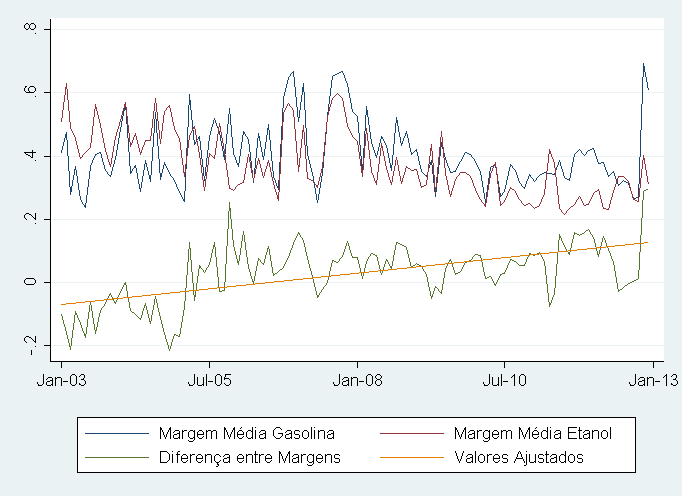
\includegraphics[width=16cm, height=10cm]{margens.png}}
\end{figure}

Sendo assim, se a diferença assumir valor zero significa que a margem de revenda dos dois produtos é idêntica. A análise do gráfico permite perceber que até a primeira metade de 2005 a margem do etanol superava a da gasolina, mas depois essa relação se inverteu. Nesse sentido, o revendedor, ao obter uma margem maior com a gasolina tende a repassar choques negativos no preço da gasolina mais rapidamente, de forma que o consumidor fique estimulado a consumir gasolina. Apesar da diferença na transmissão de preços para choques positivos, $Z^{POS}_{t-1}$, e negativos, $Z^{NEG}_{t-1}$, foi apenas o último período de análise, de janeiro de 2008 à dezembro de 2012, que apontou relativa evidência estatística de ajustamento assimétrico. A tabela \ref{teste} apresenta os p-valores referentes aos testes, tais que a hipótese nula de ajustamento simétrico pode ser rejeitada a $10\%$ no último intervalo de tempo.


\begin{table}[htbp]
  \centering
  \caption{Teste de Ajustamento Simétrico}
    \begin{tabular}{l|c|c|c}
    \toprule
     & \multicolumn{3}{c}{P-valor} \\
Variável Dependente  & \multicolumn{1}{l}{Jan 2003 à Dez 2012} & \multicolumn{1}{l}{Jan 2003 à Dez 2007} & \multicolumn{1}{l}{Jan 2008 à Dez 2012} \\ \hline
    $\Delta PR$ &  0,241      &  0,123     & 0,065  \\
    \bottomrule
    \multicolumn{4}{l}{Fonte: Elaboração Própria} \\
           \hline
    \end{tabular}%
  \label{teste}%
\end{table}%



% ----------------------------------------------------------
% Capitulo de textual  
% ----------------------------------------------------------
\section{Conclusão}

Este estudo, ao analisar a transmissão de preços permitindo a identificação de assimetrias em situações de alta ou baixa de preços em níveis superiores da cadeia, contribui para o entendimento do mercado curitibano e, talvez, brasileiro de combustíveis. A evidência encontrada de que baixas de preços são repassadas com maior velocidade no período posterior a introdução e disseminação de veículos \textit{flex-fuel} é importante e interessante, ao retratar uma possível alteração de estratégia dos revendedores de gasolina num mercado com maior substituibilidade entre os dois tipos de combustível (Gasolina e Etanol). Uma questão que poderia ser feita neste contexto seria o porquê de tal preferência por maiores margens em um tipo específico de combustível, uma vez que as revendedoras de gasolina tendem a também comercializar o etanol, mas isto fugiria a proposta deste trabalho e segue como sugestão a trabalhos futuros.

Além disso, este estudo contribui para a literatura de assimetria de transmissão de preços, ao observar um mercado que não é o primeiro objeto de estudo desta literatura. Estudos desta linha têm viés claro observado na definição de mercados alimentícios como objeto de estudo. Ao observar o mercado de combustível, uma utilidade relativamente pouco explorada desta metodologia é apresentada.

% ----------------------------------------------------------
% Capitulo de textual  
% ----------------------------------------------------------

\cleardoublepage
% ----------------------------------------------------------
% ELEMENTOS PÓS-TEXTUAIS
% ----------------------------------------------------------


% ----------------------------------------------------------
% Referências bibliográficas
% ----------------------------------------------------------

\bibliography{refcaio}

\end{document}

